
\documentclass{sigplanconf}

\usepackage{amsmath}
\usepackage{amsopn}
\usepackage{extarrows}

\usepackage{amsthm}
\usepackage{amssymb}
\usepackage{amsfonts}
%% \usepackage{geometry}
\usepackage{enumerate}
\usepackage{xcolor}
 \usepackage{url}
%% \usepackage{amsthm,amssymb,amsfonts,geometry,enumerate,xcolor,url}
%% \usepackage[sort]{cite}
\usepackage{graphicx}
\usepackage{boxedminipage}
\usepackage{multirow}

\begin{document}

\special{papersize=8.5in,11in}
\setlength{\pdfpageheight}{\paperheight}
\setlength{\pdfpagewidth}{\paperwidth}

\titlebanner{banner above paper title}        % These are ignored unless
%\preprintfooter{short description of paper}   % 'preprint' option specified.

\title{A Behavioral Type System for Memory-Leak Freedom}

\authorinfo{Qi Tan and Kohei Suenaga}
           {Kyoto University}
           {\{tanki, ksuenaga\}@fos.kuis.kyoto-u.ac.jp}


\maketitle

\newcommand\tB{\;|\;}
\newcommand\LET{\mathbf{let}\;}
\newcommand\FREE{\mathbf{free(x)}}
\newcommand\IN{\mathbf{in}\;}
\newcommand\SKIP{\mathbf{skip}}
\newcommand\NULL{\mathbf{null}}
\newcommand\IFNULL{\mathbf{ifnull}\;}
\newcommand\THEN{\mathbf{then}\;}
\newcommand\ELSE{\mathbf{else}\;}
\newcommand\Rtab{\; \; \; \;}
\newcommand\Lcc{\left(}
\newcommand\Rcc{\right)}
\newcommand\Lfc{\left\{}
\newcommand\Rfc{\right\}}
\newcommand\Lb{\left[}
\newcommand\Rb{\right]}
\newcommand\coma{,\;}
\newcommand\MALLOC{\mathbf{malloc()}}
\newcommand\Malloc{\mathbf{malloc}}
\newcommand\Free{\mathbf{free}}
\newcommand\Cirx{(x)}
\newcommand\dtb{\;\;\ \;\;\ \;\;}
\newtheorem{exmp}{Example}[section]
\newcommand\TSEQ{;\!}
\newcommand\TSKIP{\mathbf{0}}
\newcommand\OVERFLOW{\mathbf{OutOfMemory}}
\newcommand\DOM{\mathbf{Dom}}
\newcommand\FUNTYPE{\varphi}
\newcommand\bs{\backslash}
\newcommand\MEMEX{\mathbf{MemEx}}
\newtheorem{theorem}{Theorem}[section]
\newtheorem{lemma}[theorem]{Lemma}
\newtheorem{proposition}[theorem]{Proposition}
\newtheorem{corollary}[theorem]{Corollary}
\newtheorem{myDef}{Definition}
\newtheorem{remark}{Remark}[section]
\newcommand\set[1]{\{#1\}}
\newcommand\COL{\!:\!}
\newcommand\VAR{\mathbf{Var}}

\theoremstyle{definition}

\newenvironment{nospaceflalign*}
 {\setlength{\abovedisplayskip}{0pt}\setlength{\belowdisplayskip}{0pt}%
  \csname flalign*\endcsname}
 {\csname endflalign*\endcsname\ignorespacesafterend}

\section{Problem and Motivation}
In order to prevent dynamic memory-management related errors such as
memory leaks and illegal read/write/free operations to deallocated
memory cells, many static verification techniques have been
proposed~\cite{DBLP:conf/aplas/SuenagaK09,DBLP:conf/pldi/HeineL03,DBLP:conf/sigsoft/XieA05,DBLP:journals/scp/SwamyHMGJ06,DBLP:conf/sas/OrlovichR06,DBLP:conf/issta/SuiYX12}.
These analyses proposed so far mainly guarantee \emph{partial}
memory-leak freedom: All the allocated memory cells are deallocated
\emph{if a program terminates}.  Hence, these proposed verifiers will
say that a nonterminating program is safe.

In real-world programs, \emph{total} memory-leak freedom -- a program
consumes bounded number of memory cells during execution -- is an
important property (e.g., operating systems and Web servers). However,
analyses for partial memory-leak freedom is not enough for such
software that does not terminate.

\begin{exmp}\label{ex:ex1}
\begin{figure}[h]
1  \;\;$h()$= \dtb \dtb  \dtb      \dtb          \dtb $h'()$= \\
2  \dtb $\LET \; x = \MALLOC  \; \IN$ \dtb \;\;\;\;$\LET \; x = \MALLOC  \; \IN$\\
3  \dtb $\LET \; y = \MALLOC  \; \IN$ \dtb \;\;\;\; $\LET \; y = \MALLOC  \; \IN$\\
4  \dtb $\Free(x)$; $\Free(y) $;\;$h()$ \dtb \;\;\;\;\;\;$h'()$; $\Free\Cirx$; \ $\Free(y)$
\caption{Memory leaks in nonterminating programs.}
\label{ex:np}
\end{figure}
Figure~\ref{ex:np} describes partial and total memory-leak freedom.
Both \(h\) and \(h'\) are partially memory-leak free because they do
not terminate. The function \(h\) is totally memory-leak free since it
consumes at most two cells\footnote{We assume that \(\MALLOC\)
  allocates a fixed-sized block}.  However, the function \(h'\), when
it is invoked, consumes unbounded number of memory cells; hence \(h'\)
is not totally memory-leak free, which may cause overflow.
\end{exmp}

Currently, we are investigating a static verification method to prove
total memory-leak freedom, that a program consumes bounded number of
memory cells during execution.

\section{Approach}
Our method is to abstract the behavior of programs by a
\emph{behavioral type
  system}~\cite{DBLP:journals/lmcs/KobayashiSW06,DBLP:journals/tcs/IgarashiK04,DBLP:conf/esop/HondaVK98}.
Behavioral types are described by sequential processes whose actions
represent memory allocation and deallocation. For example, our type
system can assign a type
\(\mu\alpha.\Malloc\TSEQ\Malloc\TSEQ\Free\TSEQ\Free\TSEQ\alpha\) to
the function \(h\) in Figure~\ref{ex:np}.  This type expresses that
\(h\) can allocate a memory cell twice, deallocate a memory cell
twice, and then iterate this behavior.  The type assigned to \(h'\) in
Figure~\ref{ex:np} is
\(\mu\alpha.\Malloc\TSEQ\Malloc\TSEQ\alpha\TSEQ\Free;\Free\), which
expresses that \(h'\) can allocate a memory cell twice, call itself
recursively, and then deallocate a memory cell twice.  Hence, by
inspecting the inferred types (for example, by using some model
checkers), one can estimate the upper bound required to execute \(h\)
and \(h'\).

Notice that our behavioral type system includes information only about
the number and the order of allocations, deallocations, and recursive
calls; hence, the type system does not guarantee that illegal accesses
to a dangling pointer.  However, combining safe-memory-deallocation
analyses (e.g., one proposed by Suenaga and
Kobayashi~\cite{DBLP:conf/aplas/SuenagaK09}) with our behavioral type
system, we can verify safe-memory-deallocation even for nonterminating
programs.

\subsection{Language}
The definition of the language is as follows; It
is a sublanguage of Suenaga and Kobayashi~\cite{DBLP:conf/aplas/SuenagaK09}.
\[
\begin{array}{rlcl}
  s & (\mbox{statements})&::=&\SKIP \tB s_{1};s_{2} \tB *x \leftarrow y \tB \Free \Cirx \\
  & & & \tB \LET\; x = \MALLOC \; \IN \; s  \\
  %% & & & \tB \LET x = y \; \IN s \tB \LET x = \NULL \; \IN s \\
  %% & & & \tB \LET x = *y  \; \IN s \\
  & &  & \tB f(\vec{x}) \tB \IFNULL(x) \; \THEN s_{1}\; \ELSE s_{2} \\
\end{array}
\]

%% \begin{eqnarray*}
%%   x,y,z,\dots \mbox{ (variables)} &\in& \VAR\\
%%   s \mbox{ (statements)} & ::= &  \SKIP \mid s_{1};s_{2} \mid *x \leftarrow y \mid \Free(x) \\
%%   & \mid & \LET x = \MALLOC \IN s \mid \LET x = \NULL\ \IN s  \\
%%   & \mid & \LET x = y \; \IN s \mid   \LET x = *y \; \IN s \\
%%   & \mid & \IFNULL(x) \; \THEN s_{1}\; \ELSE s_{2} \mid f(\vec{x})\\
%%   d \mbox{ (proc. defs.)} & ::= & \set{f \mapsto (x_1,\dots,x_n)s}\\
%%   D \mbox{(definitions) } &::=& \langle d_1 \cup \dots \cup d_n \rangle\\
%%   P \mbox{ (programs)} &::=& \langle D, s \rangle\\
%% \end{eqnarray*}

The command $\SKIP$ does nothing; the sequence $s_{1};s_{2}$ means the
executing order of $s_{1}$ and $s_{2}$; \(*x \leftarrow y\) updates
the content of cell pointed to by \(x\) with the value \(y\); command
$\Free\Cirx$ deallocates the memory cell through the pointer $x$;
\(\LET x = \MALLOC \; \IN s\) allocates a cell pointed to by \(x\) and
then executes \(s\); $f(\vec{x})$ means a function call which receives
some parameters. Here $\vec{x}$ represents a sequence of variables
\(x_1,...,x_n\); \(\IFNULL(x)\ \THEN\ s_1\ \ELSE\ s_2\) executes
\(s_1\) if \(x\) is \(\NULL\), otherwise \(s_2\). We omit some
commands like dereferencing a pointer, let bindings and definitions
of variables, program and so on.

%% The command $\SKIP$ does nothing; the sequence $s_{1};s_{2}$ means the
%% executing order of $s_{1}$ and $s_{2}$; \(*x \leftarrow y\) updates
%% the content of cell pointed by \(x\) with the value \(y\); command
%% $\Free\Cirx$ deallocates the memory cell through the pointer $x$; the
%% command \(\MALLOC\) allocates a memory cell; \(*y\) dereferences a
%% pointer \(y\); \(\LET x = e \; \IN s\) first binds \(x\) to the value of
%% \(e\), and then executes \(s\); $f(\vec{x})$ means a function call
%% which receives some parameters. Here $\vec{x}$ represents a sequence
%% of variables \(\{x_1,...,x_n\}\);
%% \(\IFNULL(x)\ \THEN\ s_1\ \ELSE\ s_2\) executes \(s_1\) if \(x\) is
%% \(\NULL\), otherwise \(s_2\).  For simplification, we omit definitions
%% for function, program and variables.

A program \emph{leaks} memory if the program consumes unbounded number
of memory cells.  For example, see Figure~\ref{ex:np} again, \(h\)
does not leak memory, whereas \(h'\) does; the former
consumes at most two memory cells at once but the latter consumes
unbounded number of memory cells.

\subsection{Behavioral Type System}
 We define behavioral types, CCS-like processes that abstract the
 behavior of programs, as follows:
\[
\begin{array}{rlcl}
  P & (\mbox{behavioral types})&::=& {\bf 0} \tB P_{1};P_{2} \tB P_{1}+P_{2} \\
     & & & \tB \Malloc \tB \Free \tB \alpha \tB \mu\alpha.P \\
  \Gamma & (\mbox{variable type environments}) &::=& \set{x_1, x_2, \dots, x_n}\\
  \Theta & (\mbox{function type environments}) &::=& \set{f_1\COL P_1,\dots,f_n\COL P_n}\\
\end{array}
\]

The type {\bf 0} is the behavior "does nothing"; $P_{1};P_{2}$ is for
sequential execution; $P_{1}+P_{2}$ is for choice; $\Malloc$ is the
behavior of a program that allocates a memory cell exactly once;
$\Free$ is for deallocating exactly once; $\mu\alpha.P$ is the
recursive type. For example, in Figure~\ref{ex:np}, function \(h\) has
the type
\(\mu\alpha.\Malloc\TSEQ\Malloc\TSEQ\Free\TSEQ\Free\TSEQ\alpha\);
function \(h'\) has the type
\(\mu\alpha.\Malloc\TSEQ\Malloc\TSEQ\alpha\TSEQ\Free\TSEQ\Free\).  The
semantics of behavioral types is given by a labeled transition system
like \(P\xlongrightarrow{l} P'\) where \(l \in \{\Malloc, \Free\}\). We
omit the concrete definition.

The type judgment of our type system is of the form $\Theta;\Gamma\vdash s :
P$.  It reads "under environments \(\Theta\) and  \(\Gamma\) the behavior
of \(s\) is as described in \(P\)".  We design the type system so that
\(\Theta;\Gamma \vdash s : P\) implies the following property:
\begin{quotation}
  When \(s\) executes \(\Malloc\) (resp. \(\Free\)), then there is
  \(P'\) such that \(P\xlongrightarrow{\Malloc} P'\)
  (resp. \(P\xlongrightarrow{\Free}P'\)) and \(\Theta;\Gamma \vdash s'
  : P'\), where \(s'\) is the continuation of \(s\).
\end{quotation}
This property guarantees that the behavioral types soundly
approximate the upper bound of the consumed memory cells.

We present two typing rules. 
\begin{figure}[t]
$$ \frac{}
{\Theta;\Gamma \vdash \Free() : \Free} 
\Rtab \mbox{(T-Free)} $$
$$ \frac{\Theta;\Gamma \vdash s : P}
{\Theta;\Gamma \vdash \LET x = \MALLOC \; \IN s  : \Malloc;P} 
\Rtab \mbox{(T-Malloc)} $$
\caption{Typing rules for $\Free()$ and $\MALLOC$ }
\end{figure}
%\textbf{TODO: Explanation of typing rules here}
The rule $\mbox{T-Free}$ represents that the behavior of \(\Free()\)
is \(\Free\). The rule $\mbox{T-Malloc}$ represents that \(\LET\ x =
\MALLOC\ \IN\ s\) has the behavior \(\MALLOC;P\), where \(P\) is the
behavior of \(s\).

\section{Experiment}
To check feasibility of our behavioral type system for verification of
total memory-leak freedom and investigate problems in the current type
system, we apply CPAChecker~\cite{beyer2011cpachecker} to an original
program and to a program which represents the abstracted behavior
types

\begin{figure}[!hbp]
\centering 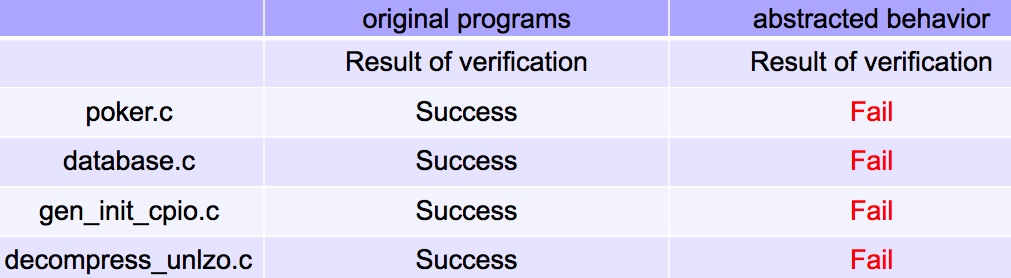
\includegraphics[width=0.5\textwidth]{exp.png}
\caption{Verification of total memory-leak free}
\label{figexp} 
\end{figure}

In Figure~\ref{figexp}, the result of verification \texttt{Success}
and \texttt{Fail} represent a program is memory-leak free and not
respectively. It shows that our behavioral type system is too
imprecise to verify total memory-leak freedom of the programs. The
reason is that our method is not path-sensitive. Figure~\ref{ex:fail}
shows this situation.
\begin{figure}[h]
\begin{verbatim}
while (...) {
   if(/* some condition c */) {
      x = malloc(sizeof(int));
   }
  /* Do something */
  if (/* condition equivalent to c  */) {
    free(x);
   }
}
\end{verbatim}
\caption{Example for path-sensitive}
\label{ex:fail}
\end{figure}

The program above is memory-leak free if the condition \(c\) is not
changed between allocation and deallocation primitives. However, the
abstracted behavioral type of the program is
\(\mu\alpha. (\mathbf{0} + \Malloc); (\mathbf{0} + \Free); \alpha\),
which is not enough to verify memory-leak freedom.

We have checked many of source codes from Github and Linux kernel and
found that extending our behavioral type system with dependencies is
useful for our future work.

\begin{figure}[h]
  \[
  \begin{array}{rlcl}
  P &  &::=& \ldots \\
  & & &\tB \mbox{CASE(x) \{VAL\(_1\) : $P_1$; \ldots ; VAL\(_n\): $P_n$  \}}\\
\end{array}
\]
\caption{Extension to dependent types}
\label{ex:beh}
\end{figure}

Figure~\ref{ex:beh} shows the extension of current behavioral type
system with dependent types. This dependent type is the behavior of a
program which has conditional branches. By using this dependent type,
the behavioral type of program in Figure~\ref{ex:fail} is
%% \(\mu\alpha.\)\mbox{CASE(c) \{VAL\(_1\) : $\Malloc$ ; VAL\(_2\): $0$ \};}
%% \mbox{CASE(c) \{VAL\(_1\) : $\Free$ ; VAL\(_2\): $0$ \}}
\(\mu\alpha.\mbox{CASE(c)}\{\mbox{VAL}_1:\Malloc;\mbox{VAL}_2:0
\};\mbox{CASE(c)}\{ \mbox{VAL}_1:\Free;\mbox{VAL}_2:0 \};
\alpha\), which is able to check no-memory-leak.

\section{Related Works}
Many static verification methods have been
proposed~\cite{DBLP:conf/aplas/SuenagaK09,DBLP:conf/pldi/HeineL03,DBLP:conf/sigsoft/XieA05,DBLP:journals/scp/SwamyHMGJ06,DBLP:conf/sas/OrlovichR06,DBLP:conf/issta/SuiYX12}
for memory-leak freedom. These methods guarantee partial memory-leak
freedom and no illegal accesses to deallocated cells.  Our behavioral
type system was supposed to prove total memory-leak freedom, but
failed due to lack of path-sensitive. By extending our behavioral type
system with dependent types, we expect it can guarantee total
memory-leak freedom.  Therefore, by using both their methods and our
type system, we can prove safe-memory deallocation even for
nonterminating programs.

Behavioral types are extensively studied in the context of concurrent
program
verification~\cite{DBLP:conf/esop/HondaVK98,DBLP:journals/tcs/IgarashiK04,DBLP:conf/esop/VieiraCS08,DBLP:journals/lmcs/KobayashiSW06}.
Our type system is largely inspired by one proposed by Kobayashi et
al.~\cite{DBLP:journals/lmcs/KobayashiSW06}, which guarantees that a
concurrent program accesses resources according to specification.

\section{Conclusion}
To verify memory-leak freedom for possibly nonterminating programs, we
have proposed a behavioral type system which abstracts the behavior of
programs with allocation and deallocation. Although we omit the
statement and proofs, we have proved the type soundness and have
conducted experiments to check feasibility of our approach.

The allocation primitives defined in our type system ignore the size
of the allocated block, only including the information about the
number and order of allocations and deallocations.  Hence, our
approach may see a memory-leak program as a well-typed one.
Variable-length cells will be included in our future work. For
preciseness, we are going to extend our type system with dependencies,
because our approach is not enough to check total memory-leak freedom.


\bibliographystyle{abbrvnat} \bibliography{tan}

\end{document}


%% \Begin{table}
%%   \scriptsize
%% \begin{tabular}{|c|c|c|}
%% \hline
%% & \texttt{original programs}  & \texttt{abstracted behavior}  \\
%% \hline
%% & \texttt{result of verification}  & \texttt{result of verification}  \\
%% \hline
%% \texttt{poker.c} & \texttt{Success} & \texttt{Fail} \\
%% \hline
%% \texttt{database.c} & \texttt{Success} & \texttt{Fail} \\
%% \hline
%% \texttt{gen\_init\_cpio.c} &\texttt{Success} & \texttt{Fail} \\
%% \hline
%% \texttt{decompress\_unlzo.c} &\texttt{Success} & \texttt{Fail} \\
%% \hline
%% \end{tabular}
%% \caption{Result of whether the program is total memory-leak free}
%% \label{tb:mcc}
%% \end{table}
